\chapter{Implementation}

\section{Algorithms in context}


\def \mheight {1cm}
\def \mwidth {2cm}
\definecolor{col2}{HTML}{C7BA9B}
\definecolor{col1}{HTML}{8B7C6D}
\definecolor{col3}{HTML}{F0EAB3}
\definecolor{col4}{HTML}{626072}
\definecolor{col5}{HTML}{40415B}

\tikzstyle{bx}=[
  fill, 
  minimum height=\mheight, 
  minimum width=\mwidth, 
  shape border rotate=90, 
  shape aspect=0.1,
  rounded corners=2mm
]

\tikzstyle{cld}=[
  cloud, 
  cloud puffs=15.7, 
  cloud ignores aspect, 
  minimum height=\mheight,
  minimum width=\mwidth, 
  align=center
]

\tikzstyle{dtb}=[
  fill,
  chamfered rectangle,
  chamfered rectangle xsep=2cm,
  minimum height=\mheight, 
  minimum width=\mwidth,
  rounded corners=1mm
]

%% \tikzstyle{box}[draw,minimum height=5em,minimum width=10em]

\begin{figure}
  \centering
  \begin{tikzpicture}[align=center,node distance=2cm]

    \node (database)[dtb, fill=col1]{Database};

    \node (wikidata)[bx, fill=col2, above=of database]{WikiDatabase};

    \node (analysis)[bx, fill=col2, above=of wikidata]{WikiAnalysis};

    \node (wikifetch)[bx, fill=col2, left=0.5\mwidth of analysis]{WikiRevisionScrape};

    \node (datahandle)[bx, fill=col2, right=0.5\mwidth of analysis]{WikiDataHandle};
    
    \node (intplot)[bx, fill=col2, above of=datahandle]{WikiInteractivePlot};
    
    \node (datplot)[bx, fill=col2,  right=0.5\mwidth of intplot]{WikiDataPlot};

    \node (wikicli)[bx, fill=col5, above= 3cm of analysis]{WikiCLI}; 
    
    \node (wikipedia)[cld, fill=col4, left=of wikicli]{\textit{Wikipedia
        API}};

    \draw [-] (database) -- (wikidata); 

    \draw [-] (wikidata) -- (analysis); 

    \draw [-] (wikidata) -- (wikifetch); 

    \draw [-] (wikidata) -- (datahandle); 

    \draw [-] (wikifetch) -- (wikipedia); 

    \draw [-] (datahandle) -- (intplot); 

    \draw [-] (datahandle) -- (datplot);

    \draw [-] (intplot) -- (wikicli); 

    \draw [-] (datplot.north) -- (wikicli); 

    \draw [-] (wikifetch) -- (wikicli); 

    \draw [-] (wikicli) -- (analysis); 

    \node (blob) [
      draw=col5, 
      fit= (wikidata) (datplot) (wikifetch), 
      inner sep=0.4cm,
      thick,
      rounded corners=8mm
    ] {};

    \node [
      col5, 
      anchor=south east, 
      xshift=-4mm,
      yshift=4mm
    ] at (blob.south east) {\textbf{the WikiRevision package}};

  \end{tikzpicture}

  \caption{Diagram showing the connections between entities in python implementation}
\end{figure}

\section{The Classes}
The project was implemented in Python, with a C++ core for the
Levenshtein distance implementation. The code runs reasonably quikly,
with it's speed mainly limited by the speed of the HTTP requests, and
the speed of the database. To compute Levenshtein distance we employ a
short C++ script that returns Python-variables, and is compiled into a
shared object library for use in Python. 

Here we discuss the five main classes in the project, and their
function in this project.

\subsection*{WikiData}
The wikidata module interfaces with the database, and maintains its
integrity. 

\subsection*{DataHandle}
In this class we find the functions that prepare the data in the
database for plotting, including weighting results if necessary. From
the CLI. 

\subsection*{WikiDataPlot}
Data Plot can be run as a script, or instantiated as a class and run
manually. Running as a script automatically runs the DumpPlot
function, picking random pages from the database to plot, as well as
reporting various metrics regarding the revisions that are currently
stored in the database. The figures used in the discussion of results
section are procduced by this function. Otherwise, the lineGraph,
barChart and trajectoryGraph functions are self-explanatory. These
files will be output from the CLI given the \textit{-p} option.

The IPlot function runs a simple PyQT widget, showing results regarding a
particular page (or a random page if unspecified). It can be run from
the CLI using the \textit{-i} argument.

\subsection*{WikiFetch}
Contains implementation of algorithm REFERENCE, including all the
necessary logical extensions to deal with CLI parameters such as the
'depth' argument, etc. It interfaces with various Wikipedia websites. 

It holds a file, scraped from the English Wikipedia, of the various
existing Wikipedia sub-domains (English (en.), German (de.), Italian
(it.), etc.), and picks it's domain name from that if asked to. This
class is engaged by the CLI.

\subsection*{WikiAnalysis}
An implementation of the algorithm found at REFERENCE. We employ
threading to speed the computation up on multi-core systems, computing
levenshtein each separate species of text in a separate thread, as
shown in figure~\ref{fig:threading}. Although (as shown in figure
FIGURE) we expect that the 'normal' text portion comparison is
inevitably longer than any non-normal, and we execute this thread last
(being the remainder text), so we would expect to be waiting on this
thread before the computation exits. Never-the-less, we found a
notable increase in performance by implementing threading.

We may extend this by allowing for that final `normal' text to be
split down into different strings, and computed in separate threads on
separate cores. We use a 'core number' variable to that end.

\begin{figure}
  \centering
  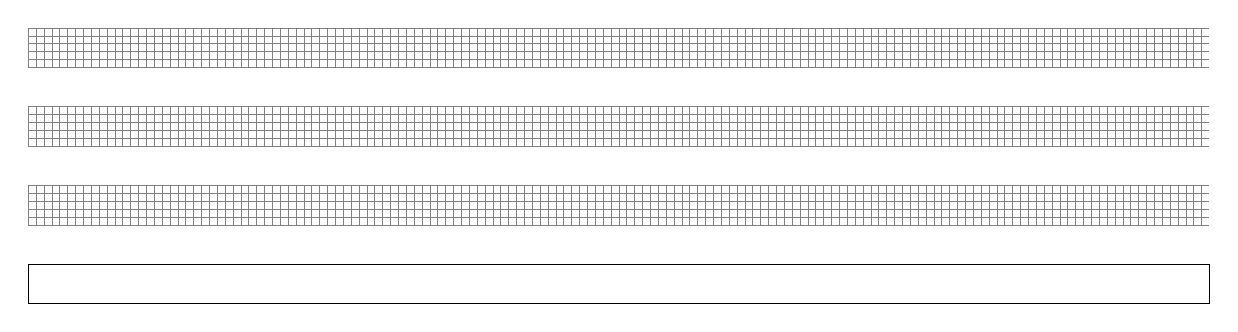
\begin{tikzpicture}[x=0.5cm, y=0.5cm]
    \draw[step=.1cm,gray,very thin] (0,6) grid (30,5);
    \draw[step=.1cm,gray,very thin] (0,4) grid (30,3);
    \draw[step=.1cm,gray,very thin] (0,2) grid (30,1);
    \draw(0,0) rectangle (30,-1);
  \end{tikzpicture}
  \caption{Diagram showing multi-processing in pair distance calculation}
\end{figure}

\section{The interface}
The CLI can be accessed using the shortcut wrhp (Wiki Revision History
Portal...). The arguments are as follows:

\begin{itemize}[label={}]
  \item \textbf{Default behvaiour.} Default behaviour is -s.
  \item \textbf{-s} Scrape and analyse. Attempts to fetch a new page
    to the database, and process it. If used with -p or -i, means to
    attempt to collect a new page from the site before plotting,
    rather than taking one from the database.
  \item \textbf{-p} Plot data. Saves png files to location given by
    the --plotpath argument.
  \item \textbf{-i} Open the interactive plot window for a given (or
    random) article once analysed.
  \item \textbf{-v} View a Wikipedia page online. Must be used with
    --domain. Can be used to view a diff (using --revid and
    --oldrevid), a specific revision (using only --revid), or the
    latest version of a page (using --pageid).
  \item \textbf{-t} `Trundle' mode. Repeats the given operation until
    interrupted. Useful for building up a database. Cannot be used
    with the --titles argument.
  \item \textbf{--title [\textit{str}]} Specify the
    pages to be scraped. Must be used with --domain. Case (and
    spelling...)  sensitive.
  \item \textbf{--domain [\textit{str}]} Specify the domain to connect
    to. May be used without --titles, limiting the random page pick to
    one domain. Must be the short version (`en', `de', etc.).
  \item \textbf{--scrapemin [\textit{int}]} Specify the minimum amount of
    pages to be scraped for one page. Default = 50.
  \item \textbf{--plotpath [\textit{filepath}]} Specify location for
    plots to be stored. Default = .
  \item \textbf{--revid} Specify the revision ID to be viewed. Used
    with -v.
  \item \textbf{--oldrevid} Specify the old revision ID when viewing a
    diff. Used with -v/
  \item \textbf{--pageid} Specify a target pageid. Can be used in -v
    and -s.
\end{itemize}
